\documentclass[UTF8,openany]{ctexbook}

% 论文版面要求:
% 统一按 word 格式A4纸(页面设置按word默认值)编排、打印、制作。
% 正文内容字体为宋体;字号为小4号;字符间距为标准;行距为25磅(约0.88175cm)。


%%%%% ===== 页面设置
\usepackage[a4paper,top=2.54cm,bottom=2.54cm,left=3.17cm,right=3.17cm,%
            ]{geometry}
\usepackage{tcolorbox}
\usepackage{fancyhdr}
\usepackage{colortbl}
\usepackage{dirtree}
\usepackage{longtable}
\usepackage{booktabs}
            
\setlength{\parindent}{2em}
%默认的弹性间距会导致文中某些排版flush的时候,出现大量空白。
\setlength{\parskip}{0.5em} %指定固定段后间距,默认为弹性间距。
\setlength{\intextsep}{10pt} %固定浮浮动体前后间距。
\usepackage{enumitem}
\usepackage{ulem}

%%%%% =====章节 标题 设置
\ctexset{%
  contentsname={\vspace{-3.5em}\centerline{\zihao{-3}\heiti 目\quad 录}\vspace{-0.7em}},
  listfigurename={\vspace{-3.5em}\centerline{\zihao{-3}\heiti 插\ 图\ 目\ 录}\vspace{-0.5em}},
  listtablename={\vspace{-3.5em}\centerline{\zihao{-3}\heiti 表\ 格\ 目\ 录}\vspace{-0.5em}},
  bibname={\vspace{-3em}\centerline{\zihao{-3}\heiti 参\ 考\ 文\ 献}\vspace{3em}},
  chapter={name={,},
  number=\arabic{chapter}, %指定章序号为一二三。。。。
  nameformat={\zihao{-2}\bfseries},
  titleformat={\zihao{-2}\bfseries},
  format=\raggedright,
  beforeskip={10pt},
  afterskip={10pt},
  pagestyle={fancy}
  },
section={format=\raggedright,
  nameformat={\zihao{4}\bfseries},
  titleformat={\zihao{4}\bfseries},
%           afterskip={1ex plus 0.2ex}
  beforeskip={1ex},% 固定段前段后间距,
  afterskip={1ex}
  },
subsection={format=\raggedright,
  nameformat={\zihao{-4}\bfseries},
  titleformat={\zihao{-4}\bfseries},
%           afterskip={0.5ex plus 0.1ex}
  beforeskip={0.5ex},
  afterskip={0.5ex}
  }
}
%%%%% ===== 中英文字体
%\setsansfont{Myriad Pro} % 无衬线字体 sans serif \sffamily
%\setmonofont{Consolas}   % 等宽字体 typewriter \ttfamily
%\newcommand{\Times}{\fontspec{Times New Roman}}
%% 中文字体
%\setCJKmainfont[BoldFont={Microsoft YaHei},ItalicFont={KaiTi}]{NSimSun}
%\setCJKsansfont{Microsoft YaHei}
%\setCJKmonofont{KaiTi}
% \setCJKfamilyfont{STSong}{方正小标宋_GBK}\newcommand{\STSong}{\CJKfamily{STSong}}
\setCJKfamilyfont{songti}{STZhongsong}\newcommand{\STSong}{\CJKfamily{STSong}}

%%%%% ===== 常用宏包
\usepackage{amsmath,amssymb,amsfonts,bm}
\usepackage[amsmath,thref,thmmarks,hyperref]{ntheorem}
\usepackage{graphicx,xcolor,float}
\usepackage{fancyhdr}
\usepackage{tocloft} % 设置目录中的条目间距


\renewcommand\cftdot{\textsubscript{……}}
\renewcommand\cftdotsep{0}

\setlength{\cftbeforechapskip}{1pt}
\renewcommand{\cftchapleader}{\cftdotfill{\cdot}}


\usepackage{booktabs} % toprule, midrule, bottomrule
\usepackage{varwidth} % 可变宽度的 parbox

%%%%% ===== 参考文献与链接
\usepackage[numbers,sort&compress,sectionbib,super, square]{natbib} %引用上标,禁用连续缩写。
\newcommand{\upcite}[1]{\textsuperscript{\cite{#1}}}


\usepackage[xetex,pagebackref]{hyperref}
\hypersetup{CJKbookmarks=true,colorlinks=true,citecolor=blue,%
            linkcolor=blue,urlcolor=blue,bookmarksnumbered=true,%
	        bookmarksopen=true,breaklinks=true}
	        
	        
	        
\iffalse   % 调试时,可去掉,以用于显示引用位置。
\renewcommand*{\backrefalt}[4]{%
\ifcase #1 No citations.%
\or Cited on page #2.%
\else Cited on pages #2.%
%\else #1 Cited on pages #2.%
\fi
}

\else
\renewcommand*{\backrefalt}[4]{}
\fi

%%%%% ===== 浮动图表的标题
\usepackage[margin=2em,labelsep=space,skip=0.5em,font=normalfont]{caption}
\DeclareCaptionFormat{mycaption}{{\heiti\color{blue} #1}#2{\kaishu #3}}
\captionsetup{format=mycaption,tablewithin=chapter,figurewithin=chapter}%,belowskip=-10pt
%\setlength{\belowcaptionskip}{-10pt}

%%%%%% ===== 浮动图表的比例默认50%以下,否则无法浮动。
\renewcommand\floatpagefraction{.9} %当浮动体小于页面90%时进行直接放置。
\renewcommand\topfraction{.9}  
\renewcommand\bottomfraction{.9}  
\renewcommand\textfraction{.1}



%%%%% ===== 算法
\usepackage{algorithm,algpseudocode}

%%%%% ===== 其他
\usepackage{ulem}
\def\ULthickness{1pt}




%%%%%===== Code Style代码
\usepackage{listings}
\usepackage{color}

\definecolor{dkgreen}{rgb}{0,0.6,0}
\definecolor{gray}{rgb}{0.5,0.5,0.5}
\definecolor{mauve}{rgb}{0.58,0,0.82}

\usepackage{accsupp}



\newcommand\emptyaccsupp[1]{\BeginAccSupp{ActualText={}}#1\EndAccSupp{}}

\lstset{
    % language = C,
    showstringspaces=false,
    xleftmargin = 3em,xrightmargin = 3em, aboveskip = 1em,
	backgroundcolor = \color{white}, % 背景色
	basicstyle = \small\ttfamily, % 基本样式 + 小号字体
	rulesepcolor= \color{gray}, % 代码块边框颜色
	breaklines = true, % 代码过长则换行
	numbers = left, % 行号在左侧显示
	numberstyle=\emptyaccsupp,
    numbersep = 14pt, 
    keywordstyle=\color{purple}\bfseries, % 关键字颜色
    commentstyle =\color{red!50!green!50!blue!60}, % 注释颜色
    stringstyle = \color{red}, % 字符串颜色
    morekeywords={ASSERT, int64_t, uint32_t},
	% frame = shadowbox, % 用(带影子效果)方框框住代码块
	frame = single, % 用(带影子效果)方框框住代码块
	showspaces = false, % 不显示空格
	columns = fixed, % 字间距固定
  framesep=1em
} 
\lstset{
    sensitive=true,
    moreemph={ASSERT, NULL}, emphstyle=\color{red}\bfseries,
    moreemph=[2]{int64_t, uint32_t, tid_t, uint8_t, int16_t, uint16_t, int32_t, size_t}, emphstyle=[2]\color{purple}\bfseries,
    showspaces = false, % 不显示空格
    }



\newcommand{\mcc}[1]{\multicolumn{1}{c}{\underline{\makebox[10em][c]{#1}}}}
\newcommand{\mce}[1]{\multicolumn{1}{c}{\underline{\makebox[15em][l]{#1}}}}


\pagestyle{fancy}
\fancyhf{}  % 清除以前对页眉页脚的设置

\newcommand{\makeheadrule}{%% 定义页眉与正文间双隔线
    \makebox[0pt][l]{\rule[.7\baselineskip]{\headwidth}{0.3pt}}%0.4
    \rule[0.85\baselineskip]{\headwidth}{1.0pt}\vskip-.8\baselineskip}
\makeatletter
\renewcommand{\headrule}{%
    % {\if@fancyplain\let\headrulewidth\plainheadrulewidth\fi\makeheadrule}}
    {\makeheadrule}}
\makeatother
\renewcommand{\chaptermark}[1]{\markboth{\CTEXthechapter \ #1}{}}
\renewcommand{\sectionmark}[1]{\markright{\thesection \ #1}{}}
%\fancyhead[RO,LE]{{\small\songti\rightmark}}     % 节标题
%\fancyhead[RE]{{\small\songti\leftmark}}      % 章标题
\fancyhead[C]{《数字图像处理》课程作业期末报告}
% \fancyhead[RO,LE]{$\cdot$ {\small\thepage} $\cdot$}
\fancyfoot[C]{{-\thepage-}}
%\fancyfoot[CO,CE]{{\thepage}}

\ctexset{chapter/break={}}

\begin{document}

\begin{titlepage}
    \begin{center}

        {
            \begin{figure}[H]
                \vspace{5cm}
                
\includegraphics[width=14cm]{img/0.png}
            \end{figure}
            \heiti\zihao{2}《数字图像处理》课程作业期末报告\\
            \vspace{1.8em}
            \zihao{2}超清视界(Vivid Restoration)\\
            \vspace{1.8em}
        }
        
        \zihao{-3}
        \begin{tabular}{p{0cm}p{0em}@{\extracolsep{0.5ex}}cc}
            ~ & \hfill             &  & \mcc{武泽恺\quad 10225101429}      \\
            ~ & \hfill             &  & \mcc{张耘彪\quad 10225101437}      \\
        \end{tabular}
        \\[8em]
        \zihao{-2}2024年7月
    \end{center}
    \thispagestyle{fancy}
    \fancyfoot[C]{}
\end{titlepage}
\fancyfoot[C]{-\thepage-}

\setcounter{page}{1}
\pagenumbering{roman}

\setcounter{page}{1}
\pagenumbering{roman}
\tableofcontents
\thispagestyle{fancy}
\newpage

\centerline{\zihao{-3}\textbf{摘\quad 要}}

\linespread{1.5}\zihao{-4} \bigskip
\kaishu
超清视界(Vivid Restoration)是一个图像增强与恢复系统,旨在通过各种图像处理技术提升图像质量。基础功能包括图像去噪、图像锐化、高通滤波以及图像形态学处理。高级功能利用Real-ESRGAN的超分辨重构技术,应用于辨别犯罪嫌疑人和拍照辅助等多种场景。

本项目GitHub仓库地址:https://github.com/Mingle-2012/picprocessing

\bigskip

\noindent{\zihao{-4}\heiti 关键词:}
图像增强,图像恢复,超分辨重构,Real-ESRGAN
\songti

\newpage
\chapter{项目背景}

随着数字技术的飞速发展,图像已成为信息传递和表达创意的重要载体。从社交媒体上的日常分享,到专业领域的科学研究、医学影像分析,再到娱乐产业的电影制作、游戏开发,图像质量对于用户体验、数据准确性以及创意表达都至关重要。然而,在实际应用中,图像往往会因为各种原因受到损伤或限制,如拍摄设备的质量不足、传输过程中的数据丢失、存储条件的恶劣以及时间的侵蚀等,导致图像分辨率低、细节模糊、色彩失真等问题。

幸运的是,我们可以借助图像增强与恢复技术弥补这些不足。这些技术旨在通过先进的算法和模型,对受损或低质量的图像进行自动修复和优化,以提升其清晰度。近年来,随着深度学习、计算机视觉等人工智能技术的突破,图像增强与恢复技术取得了显著进展,为图像质量的提升提供了强有力的支持。

正是在这样的背景下,我们开展了“超清视界(Vivid Restoration)”项目,期望通过集成数字图像基本功能和超分辨率修复模型,在利用最新的深度学习技术和图像处理算法,实现一套高效、智能的图像增强与恢复解决方案。用户可以将低质量或受损的图像转换为高清晰度的图像,从而提升用户体验。

具体来说,我们的项目将聚焦于以下几个方面:

\begin{itemize}
  \item 基于当代研发成果,构建一套完整的图像增强与恢复系统。我们采用先进的图像增强与恢复算法和模型,不断优化算法和参数设置,提升模型的处理速度和效果。

  \item 期望能够将系统应用于多个领域,如安全监控、宇航拍摄等,通过实际案例验证系统的有效性和实用性。
  
  \item 注重用户体验设计,提供简洁明了的操作界面和友好的交互方式。同时,根据用户需求提供定制化服务,满足不同场景下的图像增强与恢复需求。
\end{itemize}

\newpage

\chapter{项目介绍}

\section{项目概述}

超清视界(Vivid Restoration)系统深度融合了多种先进的图像处理技术,不仅限于基础层面的优化,还包括了高级功能的应用。我们的目标是通过图像增强与恢复技术,提升图像质量,改善图像的清晰度和细节表现,从而提升用户体验。

在基础功能层面,我们实现了图像去噪、图像锐化、图像平滑、图像形态学处理等功能,能够有效提升图像质量,改善图像的清晰度和细节表现。同时,我们还提供了用户自定义参数的接口,用户可以根据自己的需求调整参数,实现个性化的图像处理效果。

而超清视界的高级功能基于深度学习,生成对抗网络(GANs)的架构,能够学习并模拟高分辨率图像的特征,进而将低分辨率或模糊图像重建为接近原生高清甚至更高分辨率的版本。这一技术的应用,能够在图像增强与恢复领域取得显著效果。

\section{基本功能}

在基础功能层面,我们实现了以下几个功能:

\begin{itemize}
  \item 图像基本转换:
  \begin{itemize}
      \item 使用图像颜色空间转换、算术运算和几何变换等实现图像的基本转换的自由实现。
  \end{itemize}
  
  \item 图像去噪:
  \begin{itemize}
      \item 使用中值滤波、均值滤波等去噪算法,有效去除图像中的噪声,改善图像的清晰度。
  \end{itemize}
  
  \item 图像锐化:
  \begin{itemize}
      \item 采用拉普拉斯锐化等方法,增强图像边缘细节,使图像更加清晰;通过理想滤波器、巴特沃斯滤波器和高斯滤波器等高通滤波技术,增强图像的高频信息,提高图像的细节表现。
  \end{itemize}
  
  \item 图像平滑:
  \begin{itemize}
      \item 采用均值滤波、高斯滤波等方法,平滑图像,减少图像中的噪声,使图像更加清晰。
  \end{itemize}
  
  \item 图像形态学处理:
  \begin{itemize}
      \item 包括腐蚀、膨胀、开运算、闭运算等操作,用于图像边缘检测和形态学变换,增强图像的结构信息。
  \end{itemize}
\end{itemize}

对于一些功能,我们提供用户自己选择参数的接口,如图像去噪中的滤波器的参数、图像锐化中的锐化程度等,用户可以在弹出的窗口中输入自己想要的参数,以实现更加个性化的图像处理效果。

以上只是对我们所实现的功能进行了简单枚举,具体功能可以通过打开我们的软件进行体验。

\section{高级功能}

基础功能提供了十分强大而丰富的图像处理能力,但在实际应用中,我们发现对于一些特殊场景,如远距离拍摄、低分辨率图像等,基础功能的效果并不尽如人意。

同时,在介绍视频中,我们所谈到了两个明确的场景:

\begin{itemize}
  \item 太空拍摄
  \begin{itemize}
    \item 由于太空拍摄的特殊性,拍摄到的图像往往分辨率较低,且受到各种因素的影响,如尘埃、光线等,导致图像质量较差。
  \end{itemize}
  \item 犯罪嫌疑人辨识
  \begin{itemize}
    \item 在监控视频中,由于拍摄距离较远,犯罪嫌疑人的面部特征往往无法清晰辨认,给案件侦破带来困难。
  \end{itemize}
\end{itemize}

基于上述基础功能,我们可以借助图像锐化和恢复来对图像进行初步优化。借助图像锐化,我们可以增强图像的边缘细节,使图像更加清晰;借助图像恢复,我们可以去除图片的噪声,使图像更加干净。但是,这些功能仍然无法解决图像分辨率低的问题。

因此,我们引入了SRGAN的超分辨重构技术,用于解决这些特殊场景下的图像增强问题。SRGAN是一种基于生成对抗网络(GANs)的超分辨率重构技术,能够学习并模拟高分辨率图像的特征,进而将低分辨率或模糊图像重建为接近原生高清甚至更高分辨率的版本。

\newpage

\chapter{具体实现}

我们采用了\texttt{C\#}语言,使用\texttt{.NET}框架进行开发。我们使用了\texttt{OpenCV}库,实现了图像处理的基本功能,如图像去噪、图像锐化、图像平滑、图像形态学处理等。

为了开发Windows应用程序,我们使用了\texttt{WPF}框架,实现了图形用户界面。用户可以通过界面选择图像处理的功能和参数,实现对图像的处理。

\section{基础功能实现}

在实现过程中,我们进行了实现接口与调用接口的分离,使得系统更加灵活,易于扩展。同时,我们还进行了代码的模块化设计,使得代码更加清晰易懂,易于维护。

以下是我们所实现的主要接口:

\begin{enumerate}[label=\arabic*., leftmargin=*]

  \item \textbf{图像加载与显示}
    \begin{itemize}[label=--, leftmargin=*]
      \item \texttt{LoadImage}方法用于加载图像。
      \item \texttt{ShowImage}和\texttt{ShowImageNoWait}方法用于显示图像,后者可以用于一次性显示多张图片。
    \end{itemize}
  
  \item \textbf{图像颜色空间转换}
    \begin{itemize}[label=--, leftmargin=*]
      \item \texttt{ToHsv}方法将图像从BGR转换为HSV。
      \item \texttt{ToGray}方法将彩色图像转换为灰度图像。
    \end{itemize}
  
  \item \textbf{图像算术运算}
    \begin{itemize}[label=--, leftmargin=*]
      \item 提供了图像按位与(\texttt{And})、按位或(\texttt{Or})、加法(\texttt{Add})、减法(\texttt{Sub})、乘法(\texttt{Mul})和除法(\texttt{Div})等运算。
    \end{itemize}
  
  \item \textbf{图像几何变换}
    \begin{itemize}[label=--, leftmargin=*]
      \item \texttt{Resize}方法用于调整图像大小。
      \item \texttt{Rotate}方法用于旋转图像。
      \item \texttt{Translate}方法用于平移图像。
      \item \texttt{Flip}方法用于翻转图像。
    \end{itemize}
  
  \item \textbf{频域变换}
    \begin{itemize}[label=--, leftmargin=*]
      \item \texttt{RealDft}方法用于进行离散傅里叶变换,返回图像的频谱图。
    \end{itemize}
  
  \item \textbf{灰度变换}
    \begin{itemize}[label=--, leftmargin=*]
      \item 提供了对数变换(\texttt{LogTransform})和线性变换(\texttt{LinearTransform})的方法。
    \end{itemize}
  
  \item \textbf{直方图均衡}
    \begin{itemize}[label=--, leftmargin=*]
      \item \texttt{HistNormalize}和\texttt{EqualizeHist}方法用于进行直方图均衡。
    \end{itemize}
  
  \item \textbf{图像阈值化}
    \begin{itemize}[label=--, leftmargin=*]
      \item \texttt{Threshold}方法用于图像的阈值化处理。
    \end{itemize}
  
  \item \textbf{霍夫变换}
    \begin{itemize}[label=--, leftmargin=*]
      \item 实现了霍夫变换来检测直线。首先对图像进行高斯模糊,然后使用Canny边缘检测,再通过霍夫变换检测直线并绘制到结果图像上。
    \end{itemize}
  
  \item \textbf{概率霍夫变换}
    \begin{itemize}[label=--, leftmargin=*]
      \item \texttt{HoughLinesP}方法与\texttt{HoughLines}类似,但使用的是概率霍夫变换,检测到的线段是有限长度的。
    \end{itemize}
  
  \item \textbf{Robert算子边缘检测}
    \begin{itemize}[label=--, leftmargin=*]
      \item 首先将图像转换为灰度图像,然后使用Roberts算子分别在x和y方向进行卷积,最后合并结果得到边缘检测图像。
    \end{itemize}
  
  \item \textbf{Sobel算子边缘检测}
    \begin{itemize}[label=--, leftmargin=*]
      \item 与Roberts算子类似,但Sobel算子在x和y方向上的卷积核更大,能更好地捕捉边缘。
    \end{itemize}
  
  \item \textbf{拉普拉斯算子边缘检测}
    \begin{itemize}[label=--, leftmargin=*]
      \item 拉普拉斯算子是一种二阶导数算子,函数中使用拉普拉斯算子捕捉图像中的边缘。
    \end{itemize}
  
  \item \textbf{高斯-拉普拉斯算子边缘检测}
    \begin{itemize}[label=--, leftmargin=*]
      \item 首先对图像进行高斯模糊,然后使用自定义卷积核进行卷积操作。
    \end{itemize}
  
  \item \textbf{Canny边缘检测}
    \begin{itemize}[label=--, leftmargin=*]
      \item 使用Canny边缘检测算法进行多级边缘检测。
    \end{itemize}
  
  \item \textbf{均值滤波器}
    \begin{itemize}[label=--, leftmargin=*]
      \item 使用均值滤波器对图像进行平滑处理,通过取邻域内像素的平均值来平滑图像,去除噪声。
    \end{itemize}
  
  \item \textbf{理想低通滤波器}
    \begin{itemize}[label=--, leftmargin=*]
      \item 首先对图像进行傅里叶变换,然后应用低通滤波器,最后进行逆傅里叶变换得到滤波后的图像。
    \end{itemize}
  
  \item \textbf{巴特沃斯低通滤波器}
    \begin{itemize}[label=--, leftmargin=*]
      \item 与理想低通滤波器类似,但Butterworth滤波器在截止频率附近有更平滑的过渡。
    \end{itemize}
  
  \item \textbf{高斯低通滤波器}
    \begin{itemize}[label=--, leftmargin=*]
      \item 与理想和Butterworth滤波器不同,高斯滤波器使用高斯函数来平滑地截断高频分量。
    \end{itemize}
  
  \item \textbf{高斯-拉普拉斯算子边缘检测}
    \begin{itemize}[label=--, leftmargin=*]
      \item 首先对图像进行高斯模糊,然后使用拉普拉斯算子检测边缘。
    \end{itemize}
  
  \item \textbf{锐化}
    \begin{itemize}[label=--, leftmargin=*]
      \item 用拉普拉斯算子锐化图像,通过计算每个像素的周围像素的差异来增强边缘和细节。
    \end{itemize}
  
  \item \textbf{高通滤波}
    \begin{itemize}[label=--, leftmargin=*]
      \item 首先对图像进行傅里叶变换,应用高通滤波器,最后进行逆傅里叶变换得到滤波后的图像。
    \end{itemize}

    \item \textbf{轮廓检测}
    \begin{itemize}[label=--, leftmargin=*]
    \item 使用Canny边缘检测、阈值化或者形态学操作,找到并绘制图像中物体的轮廓。
    \end{itemize}
  
  \item \textbf{腐蚀}
    \begin{itemize}[label=--, leftmargin=*]
      \item 使用指定大小的矩形结构元素对图像进行腐蚀操作,减少图像中的白色区域。
    \end{itemize}
  
  \item \textbf{膨胀}
    \begin{itemize}[label=--, leftmargin=*]
      \item 使用指定大小的矩形结构元素对图像进行膨胀操作,增加图像中的白色区域,通常与腐蚀操作结合使用以便更好地处理图像中的物体。
    \end{itemize}

      \item \textbf{开运算}
      \begin{itemize}[label=--, leftmargin=*]
      \item 开运算是先进行腐蚀操作,然后进行膨胀操作的组合,可以用来去除小的噪声。
      \end{itemize}
      
      \item \textbf{闭运算}
      \begin{itemize}[label=--, leftmargin=*]
      \item 闭运算是先进行膨胀操作,然后进行腐蚀操作的组合,可以用来填充物体内部的小孔或裂缝。
      \end{itemize}
      
      \item \textbf{形态学梯度}
      \begin{itemize}[label=--, leftmargin=*]
      \item 形态学梯度是通过对原始图像应用膨胀和腐蚀操作,然后计算它们的差异来获取图像边缘的一种方法。
      \end{itemize}
      
      \item \textbf{图像加噪}
      \begin{itemize}[label=--, leftmargin=*]
      \item 提供了椒盐噪声。
      \end{itemize}

      \item \textbf{图像恢复}
      \begin{itemize}[label=--, leftmargin=*]
      \item 使用中值滤波器、选择滤波器等方法对图像进行去噪处理。
      \end{itemize}
\end{enumerate}

\section{高级功能实现}

\subsection{心路历程}

最初,我们选择了RGAN(Recurrent Generative Adversarial Network)进行实验。RGAN结合了循环神经网络和生成对抗网络,通过递归的方式逐步生成高分辨率图像。我们认为这种递归特性能够逐步细化图像细节,从而生成更高质量的图像。然而,在实际操作中,我们发现RGAN生成的图像虽然在大体结构上有所提升,但在细节处理上仍然不够理想,特别是在高频信息的处理上效果不佳。\cite{ref1}

比如当我们将一张高分辨率的人像进行模糊化的降低分辨率处理之后给到这个大模型,最后跑出来的图片人像面部特征几乎丢失殆尽,甚至相较于原图显得更加模糊抽象,于是我们决定寻找这个模型提出之后后人进行了什么样的改进。

所以我们顺藤摸瓜找到了ESRGAN,它在SRGAN的基础上进行了改进,采用了残差-in-残差密集块(Residual-in-Residual Dense Block, RRDB),并引入了感知损失和对抗损失。实验结果显示,ESRGAN生成的图像在细节表现和整体视觉效果上有显著提升。特别是RRDB的应用,使得图像细节更加丰富,边缘更加清晰。相比于RGAN,ESRGAN在平衡全局一致性和细节处理方面表现得更加出色。\cite{ref2}

尽管ESRGAN在效果上已经有了显著的提升,但我们仍然希望进一步优化模型,以达到更好的效果,于是我们惊喜地找到了Real-ESRGAN并进行了尝试。Real-ESRGAN在ESRGAN的基础上,针对实际应用中的降质模型进行了进一步的优化,特别是在处理实际拍摄的低质量图像时表现更加稳健。实验中,Real-ESRGAN生成的图像不仅在细节上非常丰富,而且在处理复杂背景和多样化图像质量时也能保持较高的稳定性。\cite{ref3}

\subsection{Real-ESRGAN模型训练}

下面,我们将介绍Real-ESRGAN模型训练过程。

1.下载数据集

\begin{figure}[H]
  \centering
  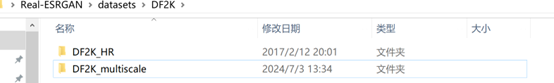
\includegraphics[width=0.8\textwidth]{img/1.png}
  \caption{下载数据集}
\end{figure}

2.生成多重规模图像

\begin{figure}[H]
  \centering
  
\includegraphics[width=0.8\textwidth]{img/2.png}
  \caption{生成多重规模图像}
\end{figure}

运行过程如下:
\begin{figure}[H]
  \centering
  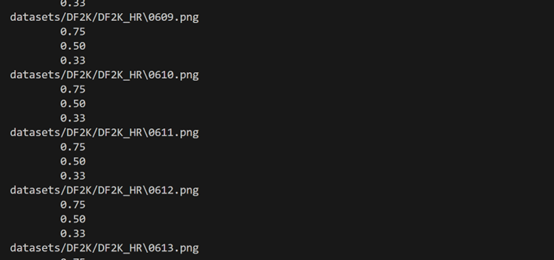
\includegraphics[width=0.8\textwidth]{img/3.png}
  \caption{生成多重规模图像}
\end{figure}

3.裁剪到子图像

\begin{figure}[H]
  \centering
  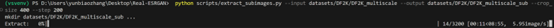
\includegraphics[width=0.8\textwidth]{img/4.png}
  \caption{裁剪到子图像}
\end{figure}

\begin{figure}[H]
  \centering
  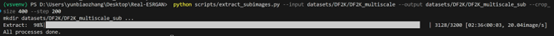
\includegraphics[width=0.8\textwidth]{img/5.png}
  \caption{裁剪到子图像}
\end{figure}

4.为元信息准备一个txt

\begin{figure}[H]
  \centering
  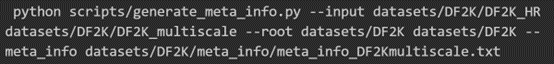
\includegraphics[width=0.8\textwidth]{img/6.png}
  \caption{为元信息准备一个txt}
\end{figure}

\begin{figure}[H]
  \centering
  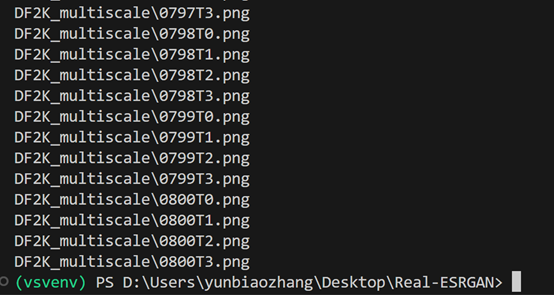
\includegraphics[width=0.8\textwidth]{img/7.png}
  \caption{为元信息准备一个txt}
\end{figure}

5.修改设置文件

\begin{figure}[H]
  \centering
  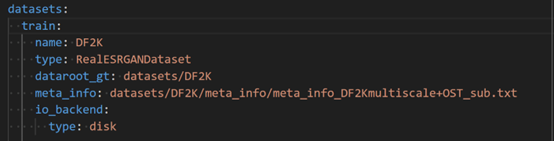
\includegraphics[width=0.8\textwidth]{img/8.png}
  \caption{修改设置文件}
\end{figure}

6.下载预训练模型
\texttt{RealESRGAN\_x4plus.pth}

\begin{figure}[H]
  \centering
  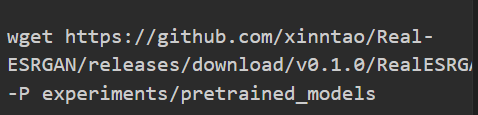
\includegraphics[width=0.8\textwidth]{img/9.png}
  \caption{下载预训练模型}
\end{figure}

\texttt{RealESRGAN\_x4plus\_netD.pth}

\begin{figure}[H]
  \centering
  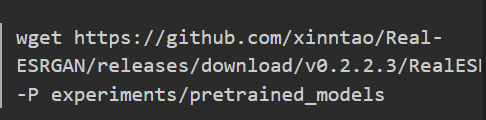
\includegraphics[width=0.8\textwidth]{img/10.png}
  \caption{下载预训练模型}
\end{figure}

7.开始训练

\begin{figure}[H]
  \centering
  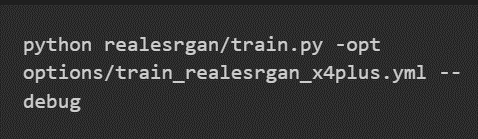
\includegraphics[width=0.8\textwidth]{img/11.png}
  \caption{开始训练}
\end{figure}

\begin{figure}[H]
  \centering
  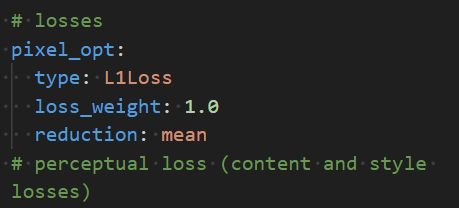
\includegraphics[width=0.8\textwidth]{img/12.png}
  \caption{开始训练}
\end{figure}

\begin{figure}[H]
  \centering
  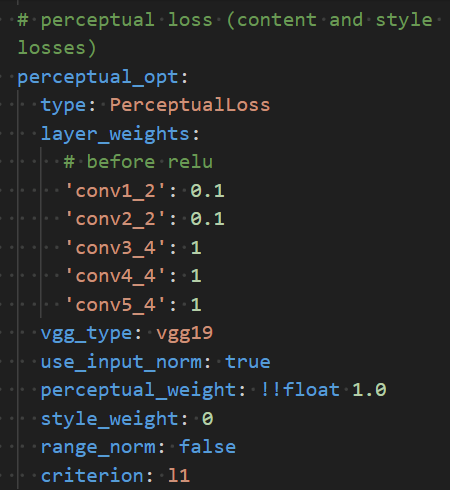
\includegraphics[width=0.8\textwidth]{img/13.png}
  \caption{开始训练}
\end{figure}

\begin{figure}[H]
  \centering
  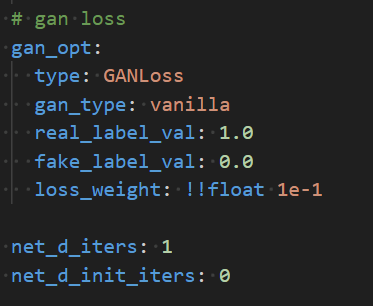
\includegraphics[width=0.8\textwidth]{img/14.png}
  \caption{开始训练}
\end{figure}

在文件中看到这三个损失作为衡量标准,于是我们去论文中看他们的含义。

\begin{itemize}
  \item L1 Loss
  \begin{itemize}
    \item L1 损失衡量的是生成图像与真实图像之间的像素级差异。较低的 L1 损失表明生成的图像与真实图像在像素值上更接近。监控训练过程中的 L1 损失曲线。如果 L1 损失在训练过程中逐渐减小且趋于平稳,说明模型在像素级别上的生成质量在提高。此外,我们还需要使用验证集来计算 L1 损失,避免过拟合。验证集上的 L1 损失应当也逐渐减小并趋于平稳。
  \end{itemize}
  \item Perceptual Loss
  \begin{itemize}
    \item 感知损失衡量的是生成图像与真实图像在特征空间中的差异,通常使用预训练的 VGG 网络提取特征。较低的感知损失表明生成的图像在感知上与真实图像更接近。感知损失逐渐减小且趋于平稳,说明模型在感知质量上逐渐提高。
  \end{itemize}
  \item GAN Loss
  \begin{itemize}
    \item 对抗损失衡量的是生成图像与真实图像在对抗网络(判别器)中的差异。较低的对抗损失表明生成的图像在判别器看来更接近真实图像。生成器和判别器的损失应当在某个平衡点附近波动。如果判别器损失过低,生成器损失过高,说明生成器还不够强;相反则说明判别器不够强。
  \end{itemize}
\end{itemize}

\subsection{对于数据集的调整}

根据这三条参数综合考量之后,我们又调整了我们的数据集,加入了BSD100用来覆盖自然风景的模拟,还加入了COCO数据集,对生活中的一般事物进行覆盖,又加入了有助于人脸修复的VGGFace2。
过程中发现在加入COCO数据集之后perceptual loss意外的变高,于是删去COCO数据集,考虑到原本的DF2K里面本身就包含很多common objects,推测对于不同类别的照片的预测正确性应该不会有太大影响。



\section{用户界面设计}

我们的用户界面采用了\texttt{WPF}框架,实现了图形用户界面。用户可以通过界面选择图像处理的功能和参数,实现对图像的处理。

首页提供了基础功能,包括图像加载、图像操作、图片迭代、清除缓存、图像导出等功能。点击输出可以查看处理后的图像。点击清除缓存可以清除缓存的图像。点击导出可以导出处理后的图像。

\begin{figure}[H]
  \centering
  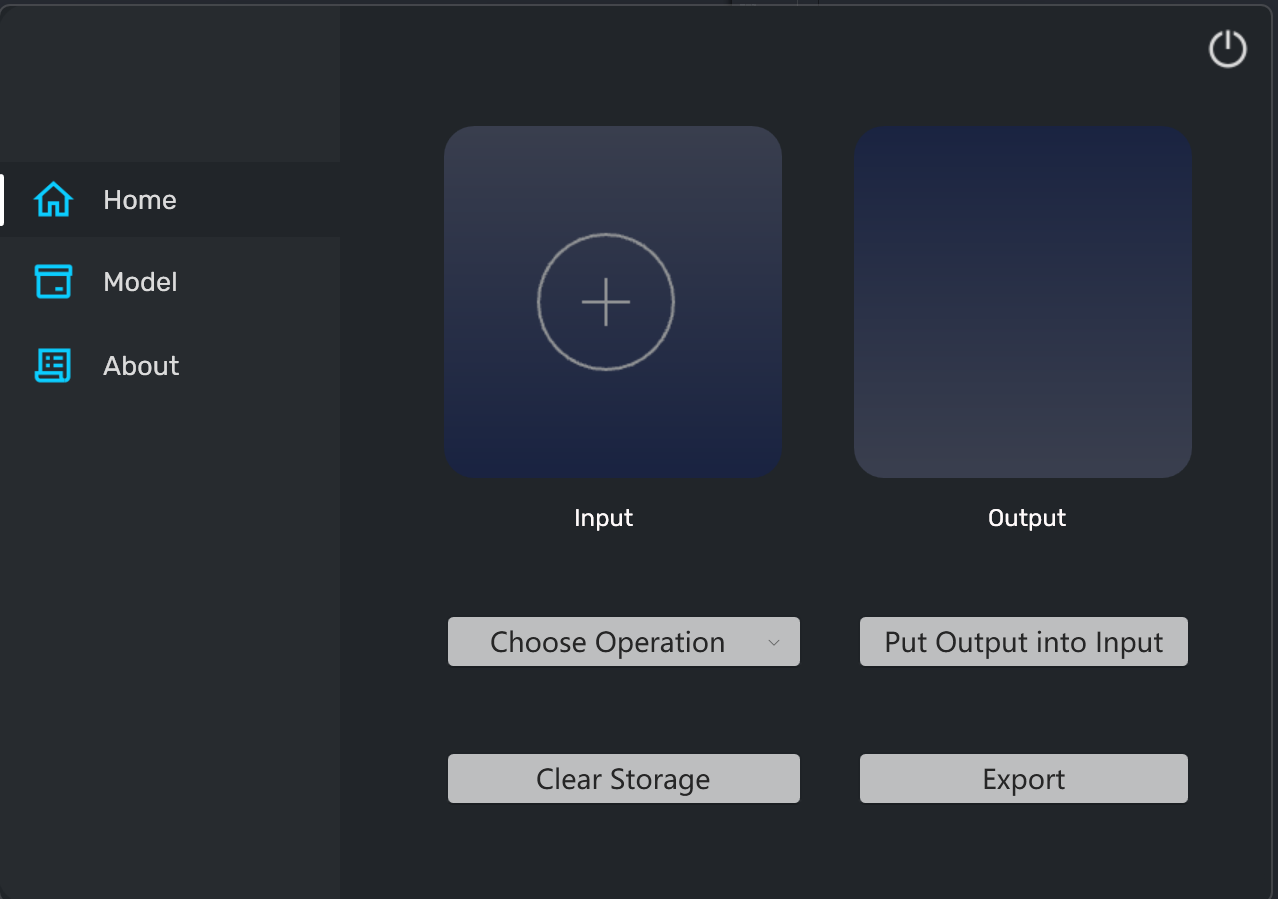
\includegraphics[width=0.8\textwidth]{img/image.png}
  \caption{首页}
\end{figure}

在选择功能时,可以打开下拉按钮选择功能。

\begin{figure}[H]
  \centering
  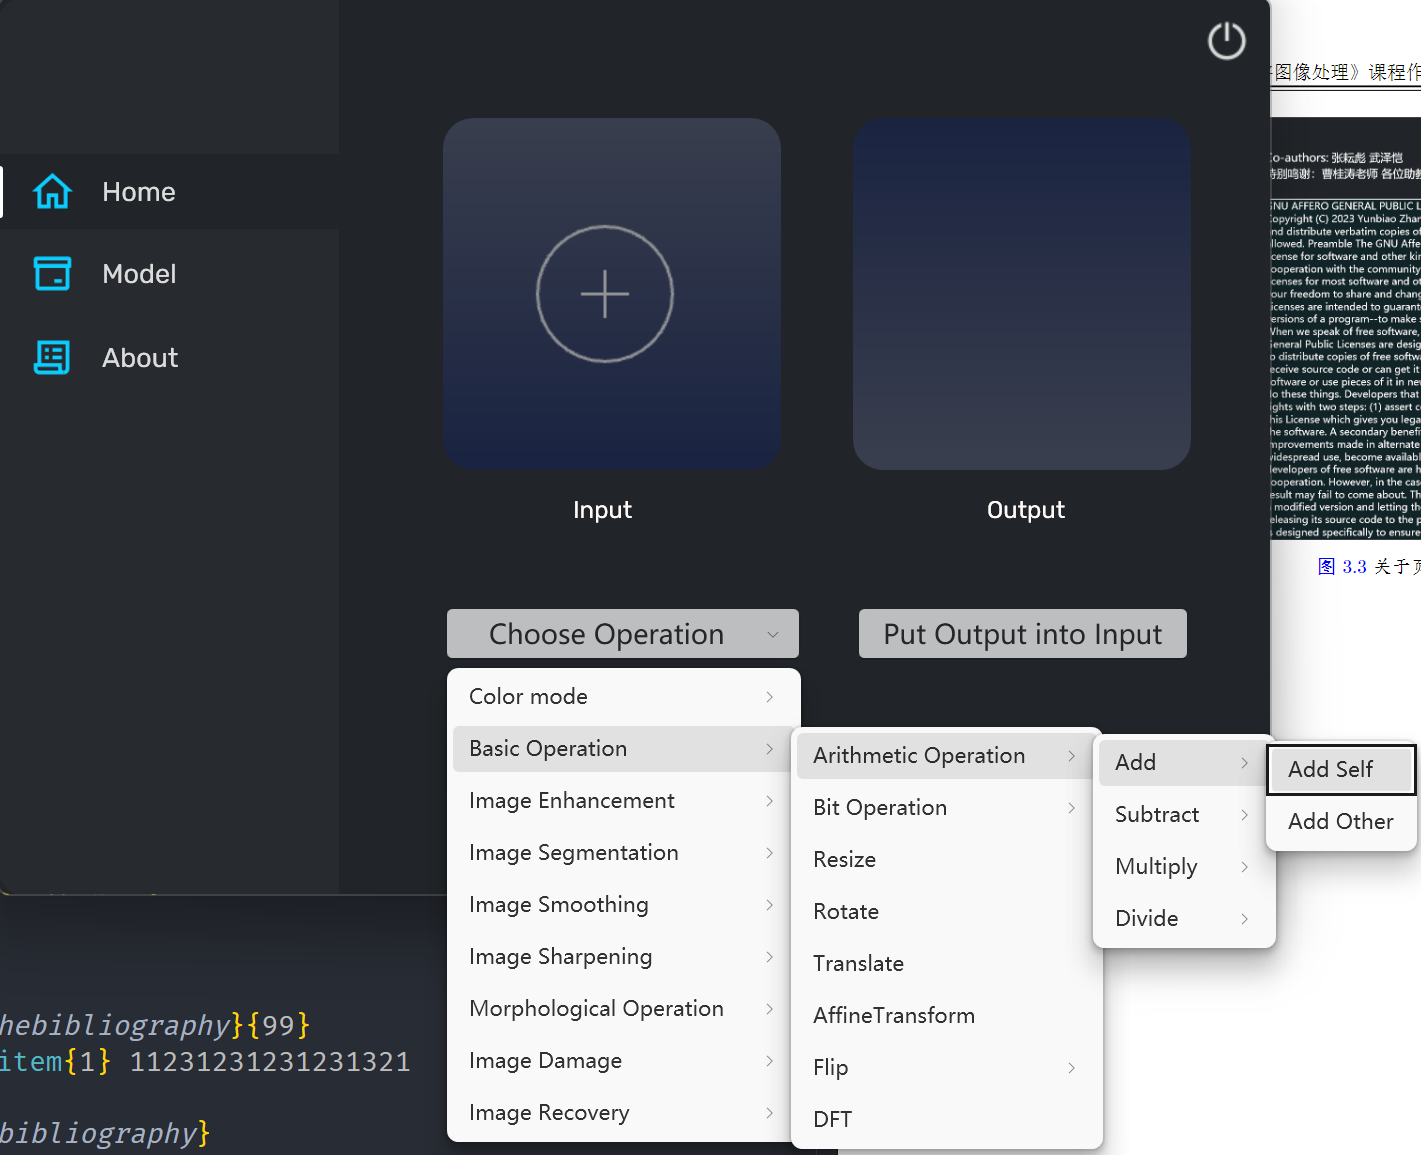
\includegraphics[width=0.8\textwidth]{img/image-3.png}
  \caption{选择功能}
\end{figure}

有些功能需要传入参数,如图像锐化的锐化程度、图像阈值化的阈值等。用户可以在弹出的窗口中输入参数,以实现更加个性化的图像处理效果。

\begin{figure}[H]
  \centering
  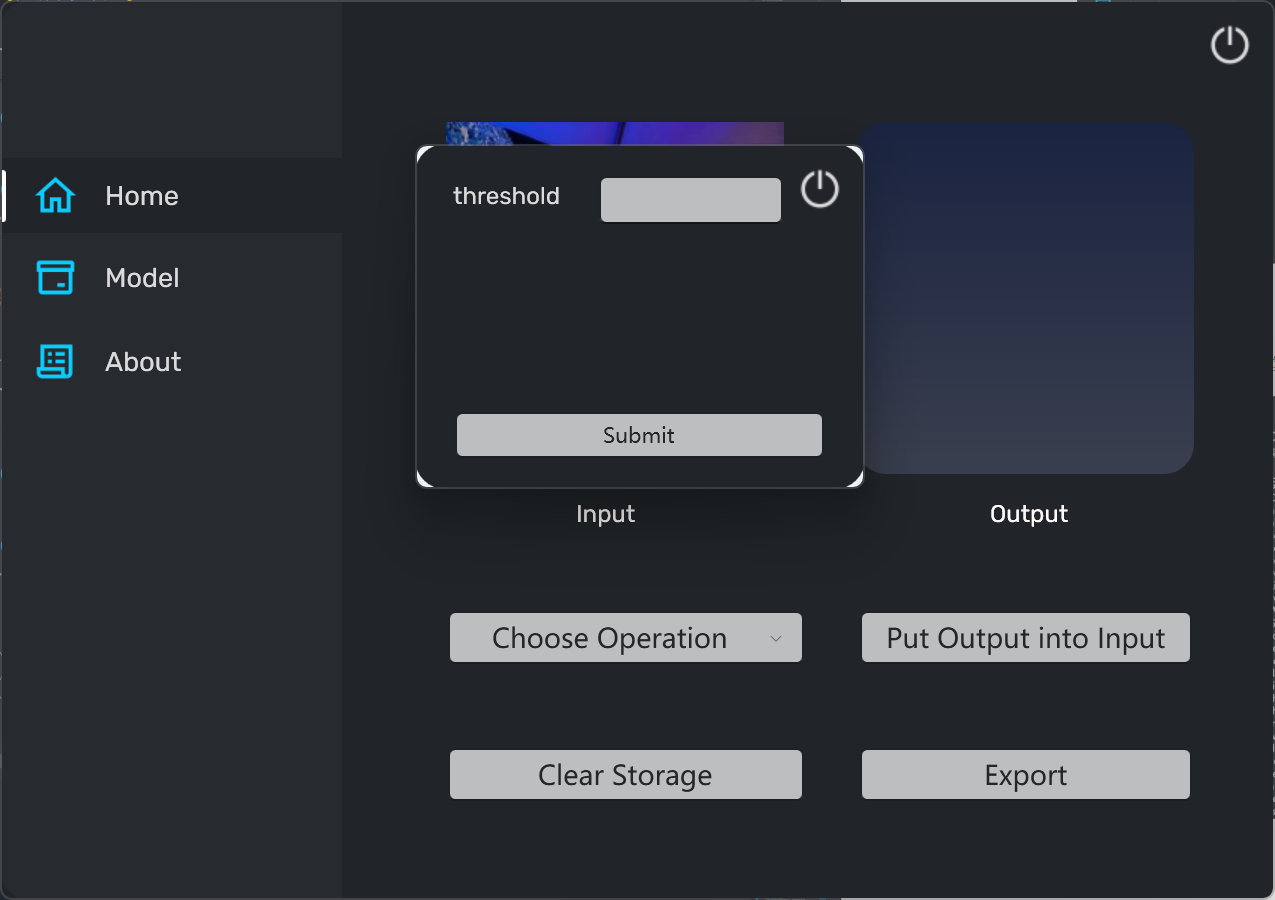
\includegraphics[width=0.8\textwidth]{img/image-4.png}
  \caption{输入参数}
\end{figure}


Model页提供了高级功能,包括彩色图片锐化修复、清除缓存、图像超分辨重构、图片导出等功能。

\begin{figure}[H]
  \centering
  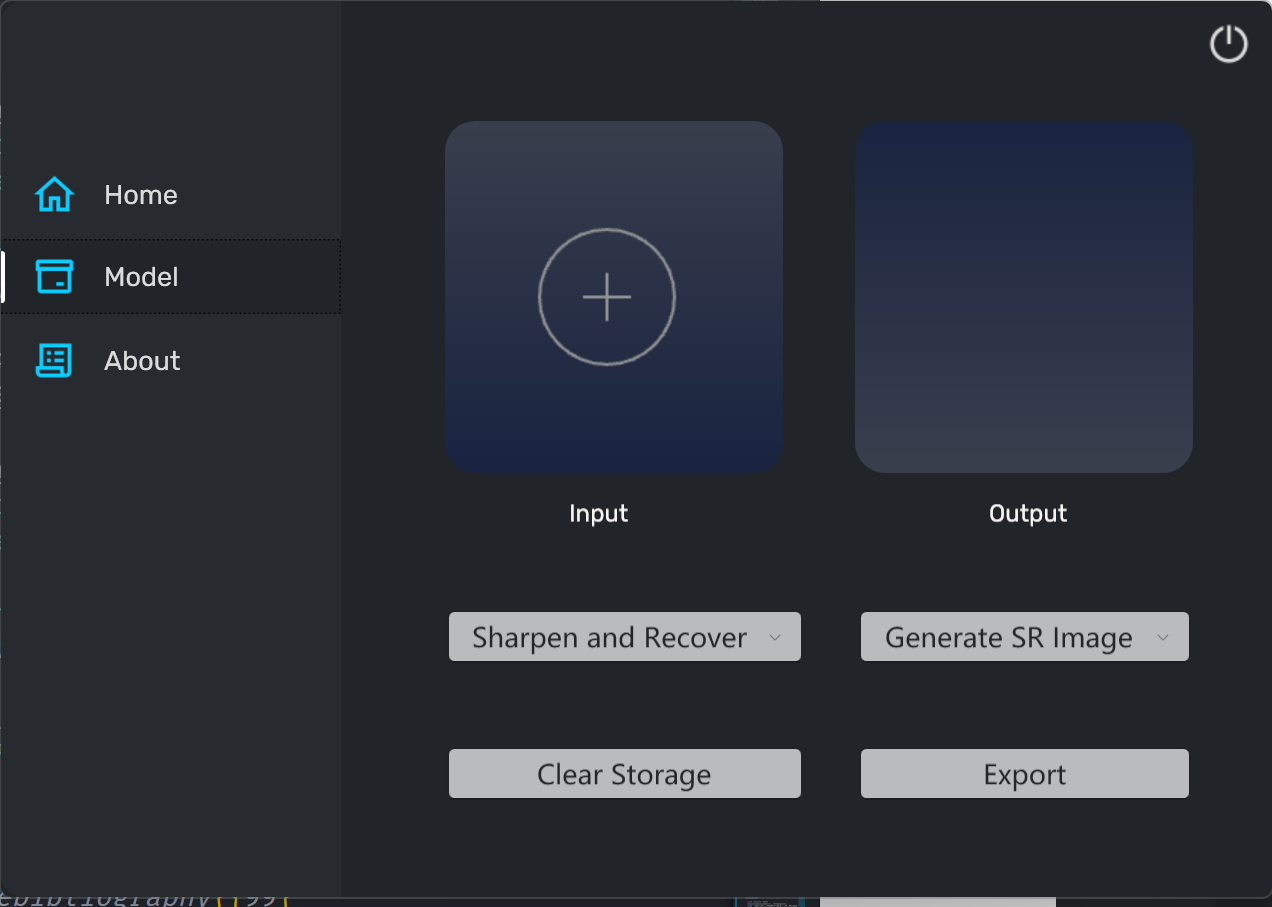
\includegraphics[width=0.8\textwidth]{img/image-1.png}
  \caption{Model页}
\end{figure}

关于页中介绍了作者,鸣谢了老师和助教老师,并声明了软件的协议。

\begin{figure}[H]
  \centering
  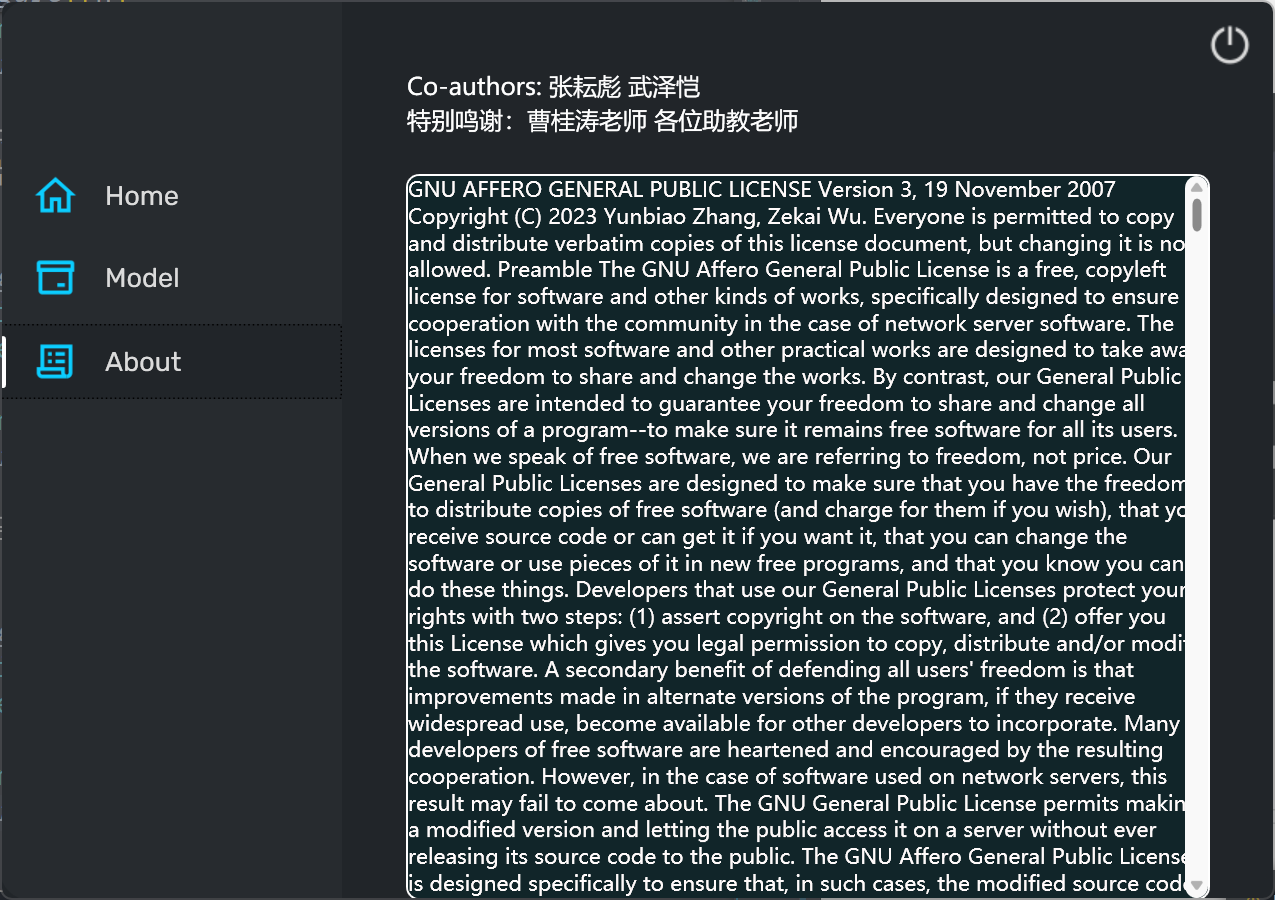
\includegraphics[width=0.8\textwidth]{img/image-2.png}
  \caption{关于页}
\end{figure}

\newpage

\chapter{总结与展望}

\section{总结}

我们所开发的超清视界(Vivid Restoration)是一个综合了多种先进数字图像处理技术的软件,包括图像去噪、图像锐化、高通滤波、图像形态学处理及超分辨率重建等多种功能,覆盖了数字图像处理的主要功能。用户可以有效去除图像中的噪声和模糊,增强图像细节,提高图像清晰度,从而满足各类应用对于高质量图像的需求。
在项目开发过程中,我们采用了OpenCV库及其相关技术,实现了各类图像处理算法的功能模块化;我们在超分辨率重建功能中,引入了基于深度学习的技术,大幅度提升了图像放大的质量与细节还原度;我们也注重了系统的用户友好性,通过提供简单明了的接口,使用户能够轻松地进行各种图像处理操作。

\section{展望}

随着科技的不断进步,图像处理技术也在不断发展和创新。我们的项目希望不断引入和集成最新的图像处理算法和技术,为用户提供更加优质的图像处理服务。

以下是对未来发展的几点展望:

\begin{itemize}[label=--]
  \item 在现有的超分辨率重建基础上,修改训练的数据集以及参数使各项 Loss 降低,或是进一步研究比 Real-SRGAN 更加准确高效的算法,使得能够使图片还原度更高,且计算代价更小。
  
  \item 目前我们只支持对图片进行处理,我们还可以优化算法的计算效率和系统性能,实现对视频的实时处理,满足更多实际应用场景的需求。
  
  \item 目前只支持 Windows 版扩展系统的跨平台能力,支持更多操作系统和设备。
  
  \item 我们期望能够提供更加灵活的用户定制功能,允许用户根据自身需求定制处理流程和参数,满足特定应用场景的要求。
\end{itemize}

  超清视界致力于提供优质的图像处理功能,我们相信通过不断的技术优化,利用数字图像处理,能够发挥越来越重要的作用,为用户创造更大的价值。

\newpage

\begin{thebibliography}{99}

  \bibitem{ref1} C. Ledig, L. Theis, F. Husz{\'a}r, J. Caballero, A. Aitken, A. Tejani, J. Totz, Z. Wang, and W. Shi, "Photo-Realistic Single Image Super-Resolution Using a Generative Adversarial Network," in \textit{Proceedings of the IEEE Conference on Computer Vision and Pattern Recognition (CVPR)}, 2017, pp. 4681--4690.
    
  \bibitem{ref2} X. Wang, K. Yu, S. Wu, J. Gu, Y. Liu, C. Dong, Y. Qiao, and C. C. Loy, "ESRGAN: Enhanced Super-Resolution Generative Adversarial Networks," in \textit{Proceedings of the European Conference on Computer Vision (ECCV) Workshops}, 2018.
    
  \bibitem{ref3} X. Wang, L. Xie, C. Dong, and Y. Shan, "Real-ESRGAN: Training Real-World Blind Super-Resolution with Pure Synthetic Data," in \textit{International Conference on Computer Vision Workshops (ICCVW)}, 2021.

\end{thebibliography}


\end{document}